\section{Auswertung}
\label{sec:Auswertung}

\subsection{Fourieranalyse}

Im ersten Versuchsteil soll der Abfall der Fourierkoeffizienten $a_k$ und $b_k$
periodischer Sägezahn, Rechtecks- und Dreiecksspannungen untersucht werden.
Dazu werden die Ordnung $k$ und die Spannungsamplitude $U$ gegeneinander
logarithmiert aufgetragen und eine lineare Regression der Form

\begin{equation}
    \text{ln} \left(U \cdot \frac{1}{\si{\volt}} \right) = a \cdot \text{ln}(k) + b
    %hier andere Beschriftung für a und b überlegen
\end{equation}

Dabei wird die Spannung $U$ durch ihre Einheit geteilt, da der Logarithmus nur für
für dimensionslose Größen definiert ist. Zudem ergibt sich umgeformt:

\begin{equation}
    U = \text{e}^b \cdot k^a \cdot \si{\volt}
    \label{eqn:Spannung}
\end{equation}

Da nun $U$ proportional zu den Fourierkoeffizienten ist, lässt sich die
Stärke deren Abfalls ermitteln.
Die Messdaten der Sägezahnspannung sind dazu in Tabelle \ref{tab:Messdaten1} aufgeführt und in 
Abbildung \ref{fig:Säge} gegeneinander aufgetragen.
Die Lineare Regression, die mittels python durchgeführt wurde, ergibt die Tangentenparameter:

\begin{align*}
    a_\text{S} &= \SI{-1.0052 \pm 0.0286}{} \\
    b_\text{S} &= \SI{07523 \pm 0.0451}{}
\end{align*}

Nach Formel \eqref{eqn:Spannung} ist zu erkennen, dass die Fourierkoeffizienten der Sägezahnspannung in etwa
proportional zu $\frac{1}{k}$ abfallen.

\begin{table}
    \centering
    \caption{Messdaten und deren Logarithmen der Sägezahnspannung}
    \label{tab:Messdaten1}
    \sisetup{table-format=2.1}
    \begin{tabular}{c c c c}
    \toprule
    $k$ & $\text{ln} (k)$ & $U \,/\, \si{\volt}$ & $\text{ln}(U \,/\, \si{\volt})$ \\
    \midrule
    1 & 0,000 & 2,040 &  0,713 \\
    2 & 0,693 & 1,100 &  0,095 \\
    3 & 1,099 & 0,740 & -0,301 \\
    4 & 1,386 & 0,488 & -0,717 \\
    5 & 1,609 & 0,440 & -0,821 \\
    6 & 1,792 & 0,352 & -1,044 \\
    7 & 1,946 & 0,296 & -1,217 \\
    8 & 2,079 & 0,280 & -1,273 \\
    9 & 2,197 & 0,216 & -1,532 \\
    \bottomrule
    \end{tabular}
\end{table} 

\begin{figure}
    \centering
    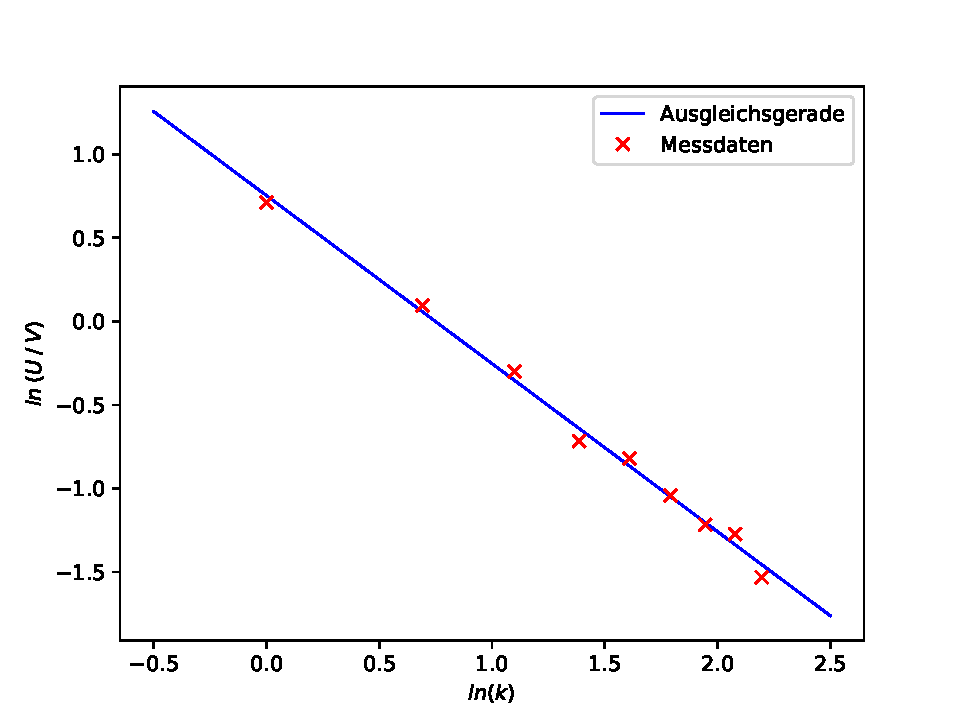
\includegraphics[scale=1.0]{content/plot1.pdf}
    \caption{Messwerte und lineare Regression für die Messwerte der Sägezahnspannung}
    \label{fig:Säge}
\end{figure}

Für die Rechtecksspannung sind die Messdaten in Tabelle \ref{tab:Messdaten2} aufgelistet und in Abbildung \ref{fig:Recht}
gegeneinander aufgetragen. Es ergeben sich die Regressionsparameter:

\begin{align*}
    a_\text{R} &= \SI{-1.0021 \pm 0.0209}{} \\
    b_\text{R} &= \SI{1.4205 \pm 0.0462}{}
\end{align*}

Nach Formel \eqref{eqn:Spannung} ist zu erkennen, dass die Fourierkoeffizienten der Rechtecksspannung in etwa
proportional zu $\frac{1}{k}$ abfallen.

\begin{table}
    \centering
    \caption{Messdaten und deren Logarithmen der Rechtecksspannung}
    \label{tab:Messdaten2}
    \sisetup{table-format=2.1}
    \begin{tabular}{c c c c}
    \toprule
    $k$ & $\text{ln} (k)$ & $U \,/\, \si{\volt}$ & $\text{ln}(U \,/\, \si{\volt})$ \\
    \midrule
    1 & 0,000 & 4,000 &  1,389 \\
    3 & 1,099 & 1,440 &  0,365 \\
    5 & 1,609 & 0,860 & -0,151 \\
    7 & 1,946 & 0,580 & -0,545 \\
    9 & 2,197 & 0,420 & -0,868 \\
   11 & 2,398 & 0,384 & -0,957 \\
   13 & 2,565 & 0,344 & -1,067 \\
   15 & 2,708 & 0,280 & -1,273 \\
   17 & 2,833 & 0,224 & -1,496 \\
   19 & 2,944 & 0,216 & -1,532 \\
    \bottomrule
    \end{tabular}
\end{table} 

\begin{figure}
    \centering
    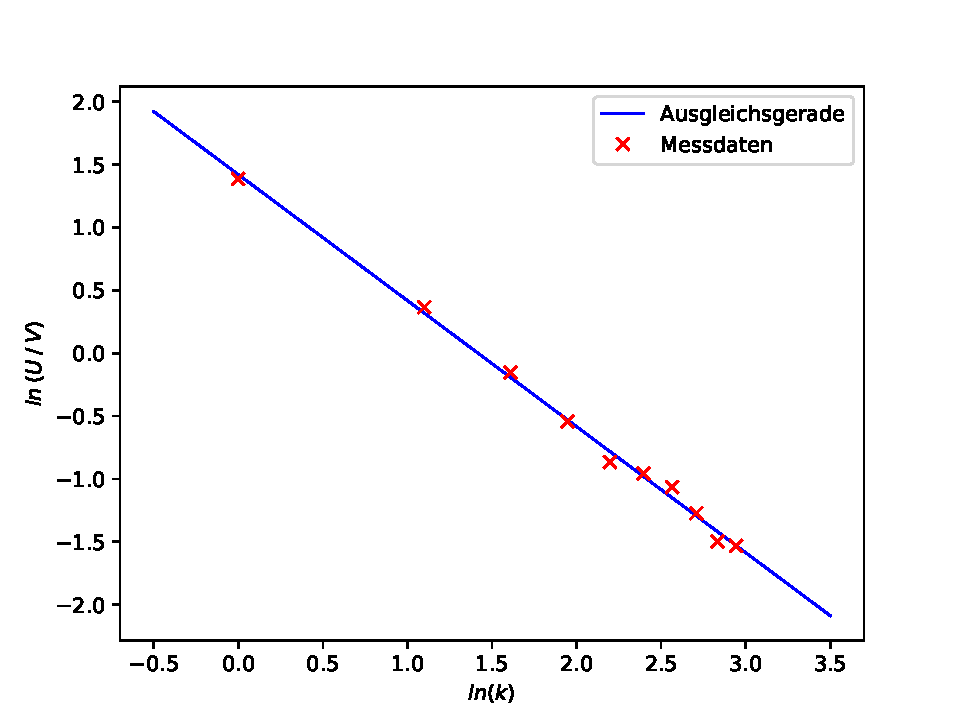
\includegraphics[scale=1.0]{content/plot2.pdf}
    \caption{Messwerte und lineare Regression für die Messwerte der Rechtecksspannung}
    \label{fig:Recht}
\end{figure}

Für die Dreiecksspannung sind die Messdaten in Tabelle \ref{tab:Messdaten3} aufgelistet und in Abbildung \ref{fig:Drei}
gegeneinander aufgetragen. Es ergeben sich die Regressionsparameter:

\begin{align*}
    a_\text{D} &= \SI{-1.9681 \pm 0.0121}{} \\
    b_\text{D} &= \SI{0.9585 \pm 0.0227}{}
\end{align*}

Nach Formel \eqref{eqn:Spannung} ist zu erkennen, dass die Fourierkoeffizienten der Dreiecksspannung in etwa
proportional zu $\frac{1}{k^2}$ abfallen.

\begin{table}
    \centering
    \caption{Messdaten und deren Logarithmen der Dreiecksspannung}
    \label{tab:Messdaten3}
    \sisetup{table-format=2.1}
    \begin{tabular}{c c c c}
    \toprule
    $k$ & $\text{ln} (k)$ & $U \,/\, \si{\volt}$ & $\text{ln}(U \,/\, \si{\volt})$ \\
    \midrule
     1 & 0,000 & 2,560 &  0,940 \\
     3 & 1,099 & 0,312 & -1,165 \\
     5 & 1,609 & 0,112 & -2,189 \\
     7 & 1,946 & 0,056 & -2,882 \\
     9 & 2,197 & 0,036 & -3,324 \\
    11 & 2,398 & 0,023 & -3,772 \\
    13 & 2,565 & 0,017 & -4,075 \\
    \bottomrule
    \end{tabular}
\end{table} 

\begin{figure}
    \centering
    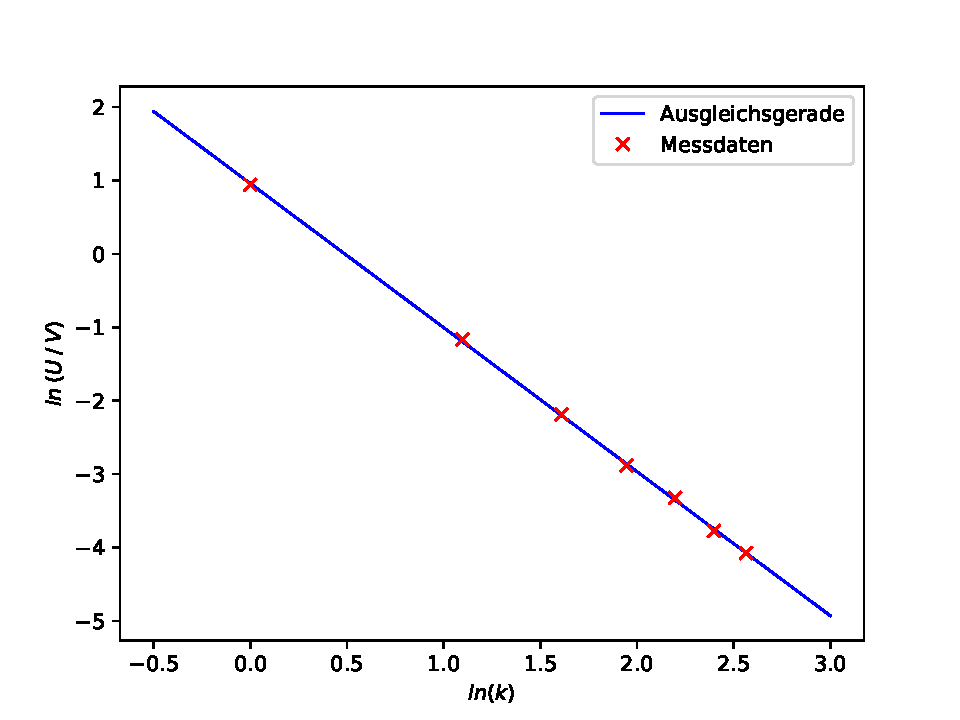
\includegraphics[scale=1.0]{content/plot3.pdf}
    \caption{Messwerte und lineare Regression für die Messwerte der Dreiecksspannung}
    \label{fig:Drei}
\end{figure}

\subsection{Fourier-Synthese}

%\begin{figure}
%    \centering
%    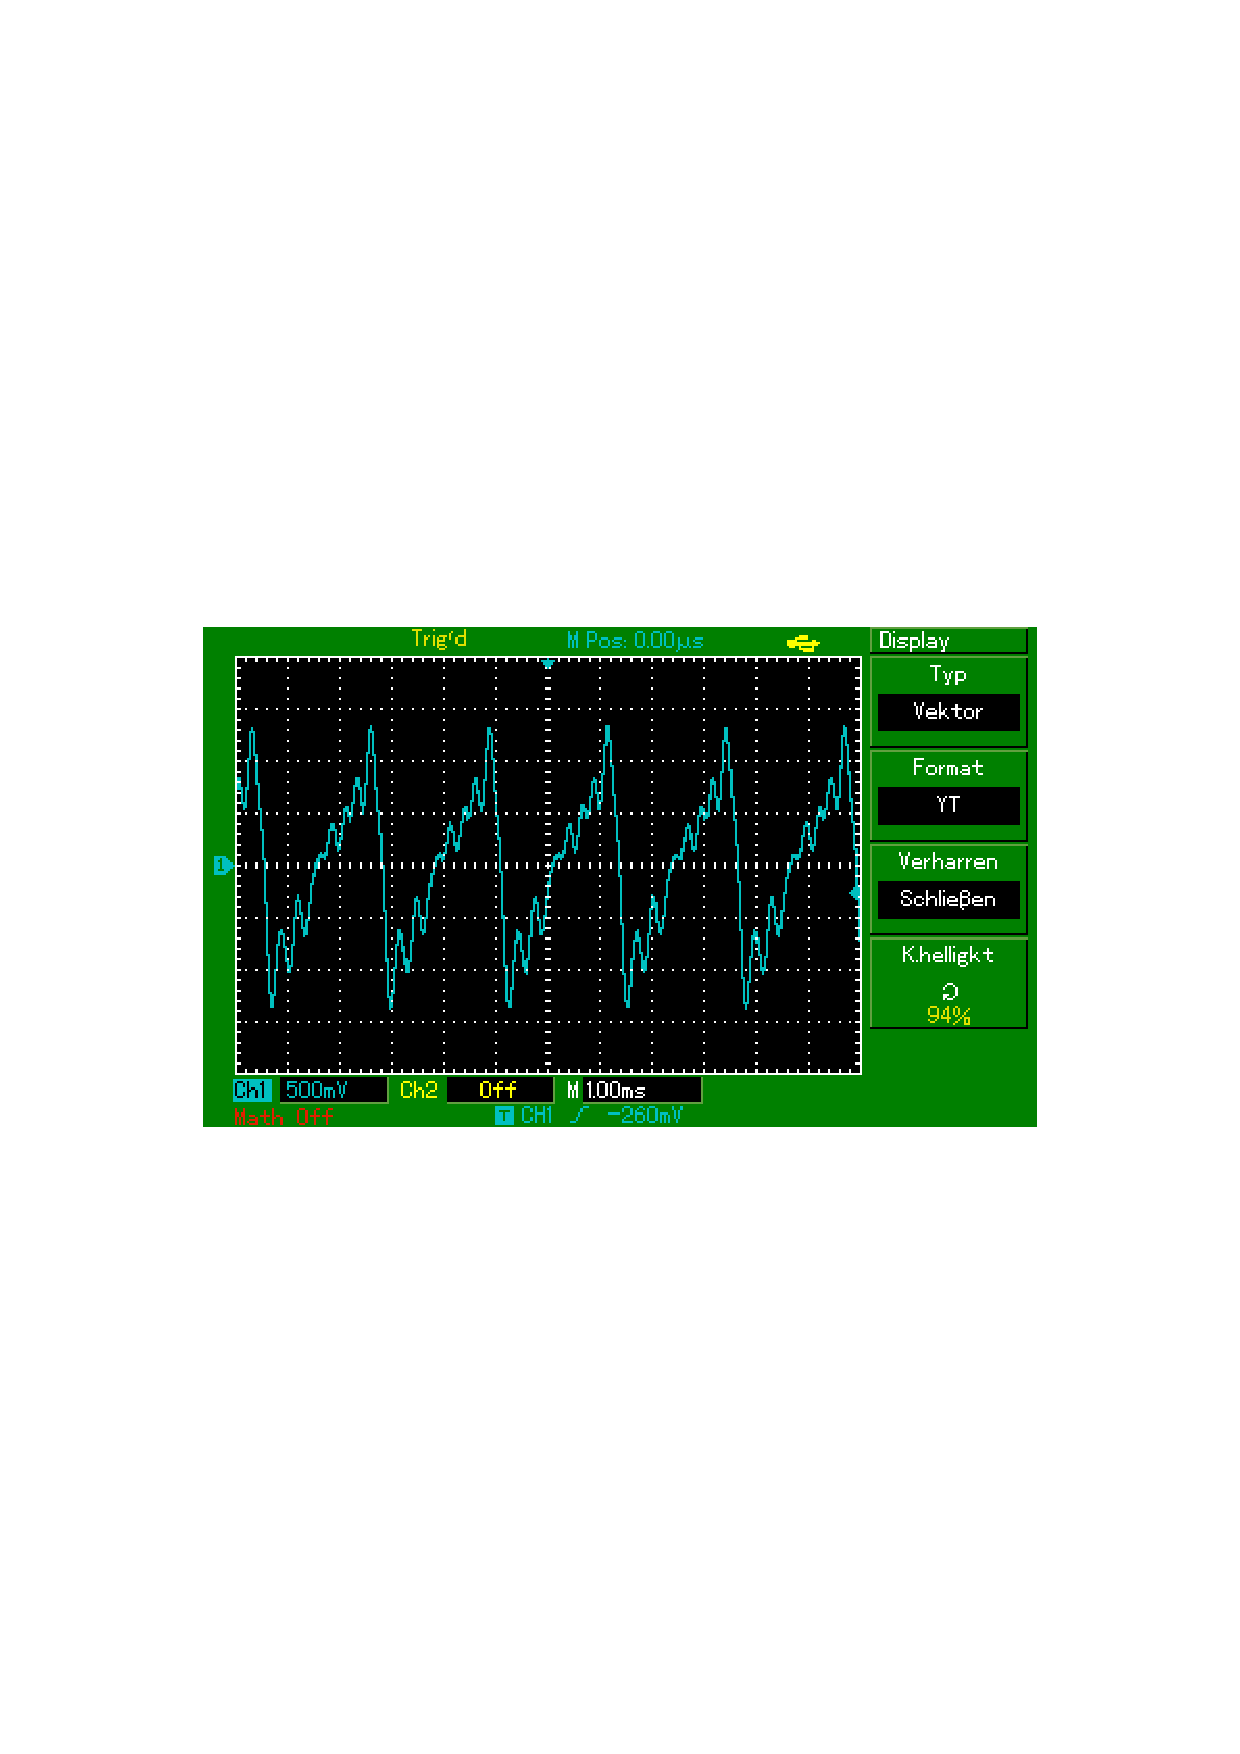
\includegraphics[scale=1.0]{content/MAP001.BMP}
%    \caption{Messwerte und lineare Regression für die Messwerte der Dreiecksspannung}
%    \label{fig:Ex1}
%\end{figure}
%
%\begin{figure}
%    \centering
%    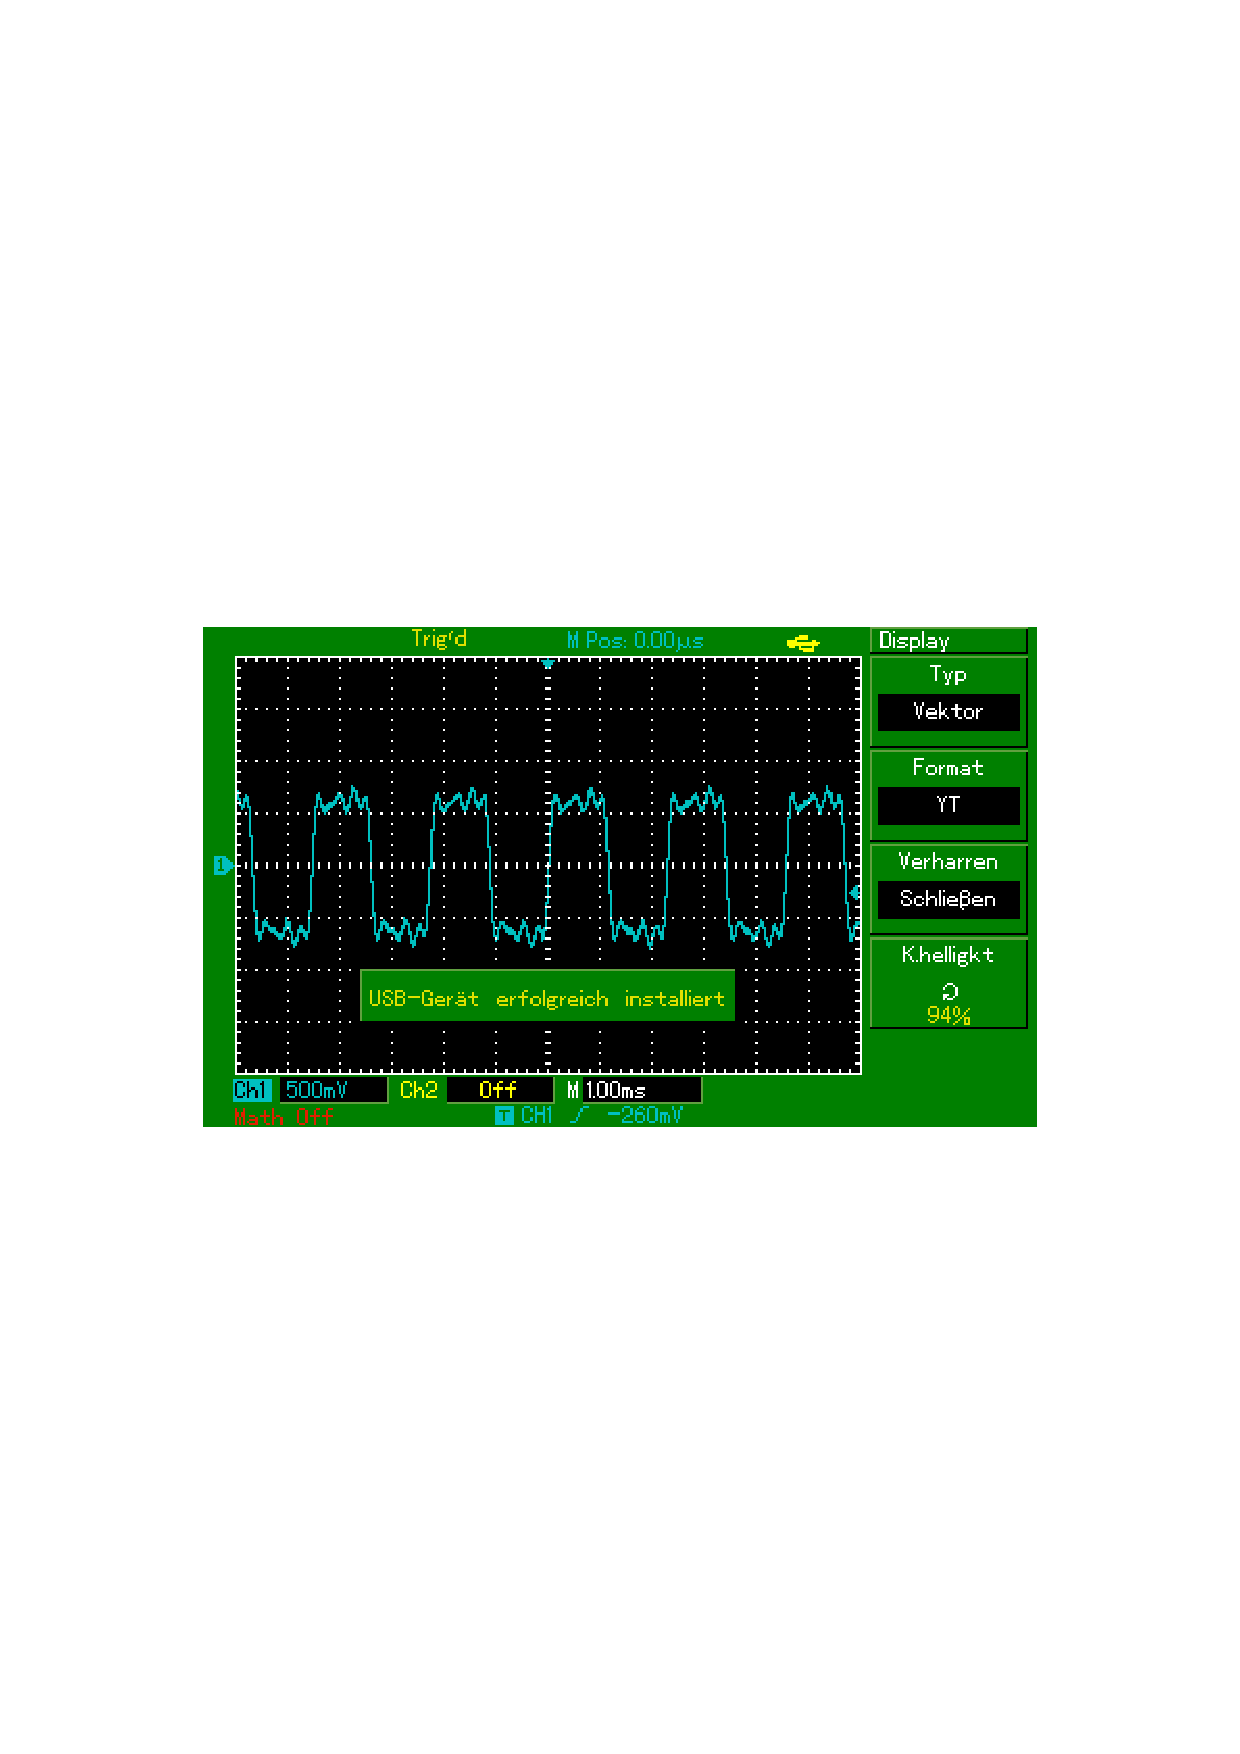
\includegraphics[scale=1.0]{content/MAP002.BMP}
%    \caption{Messwerte und lineare Regression für die Messwerte der Dreiecksspannung}
%    \label{fig:Ex2}
%\end{figure}
%
%\begin{figure}
%    \centering
%    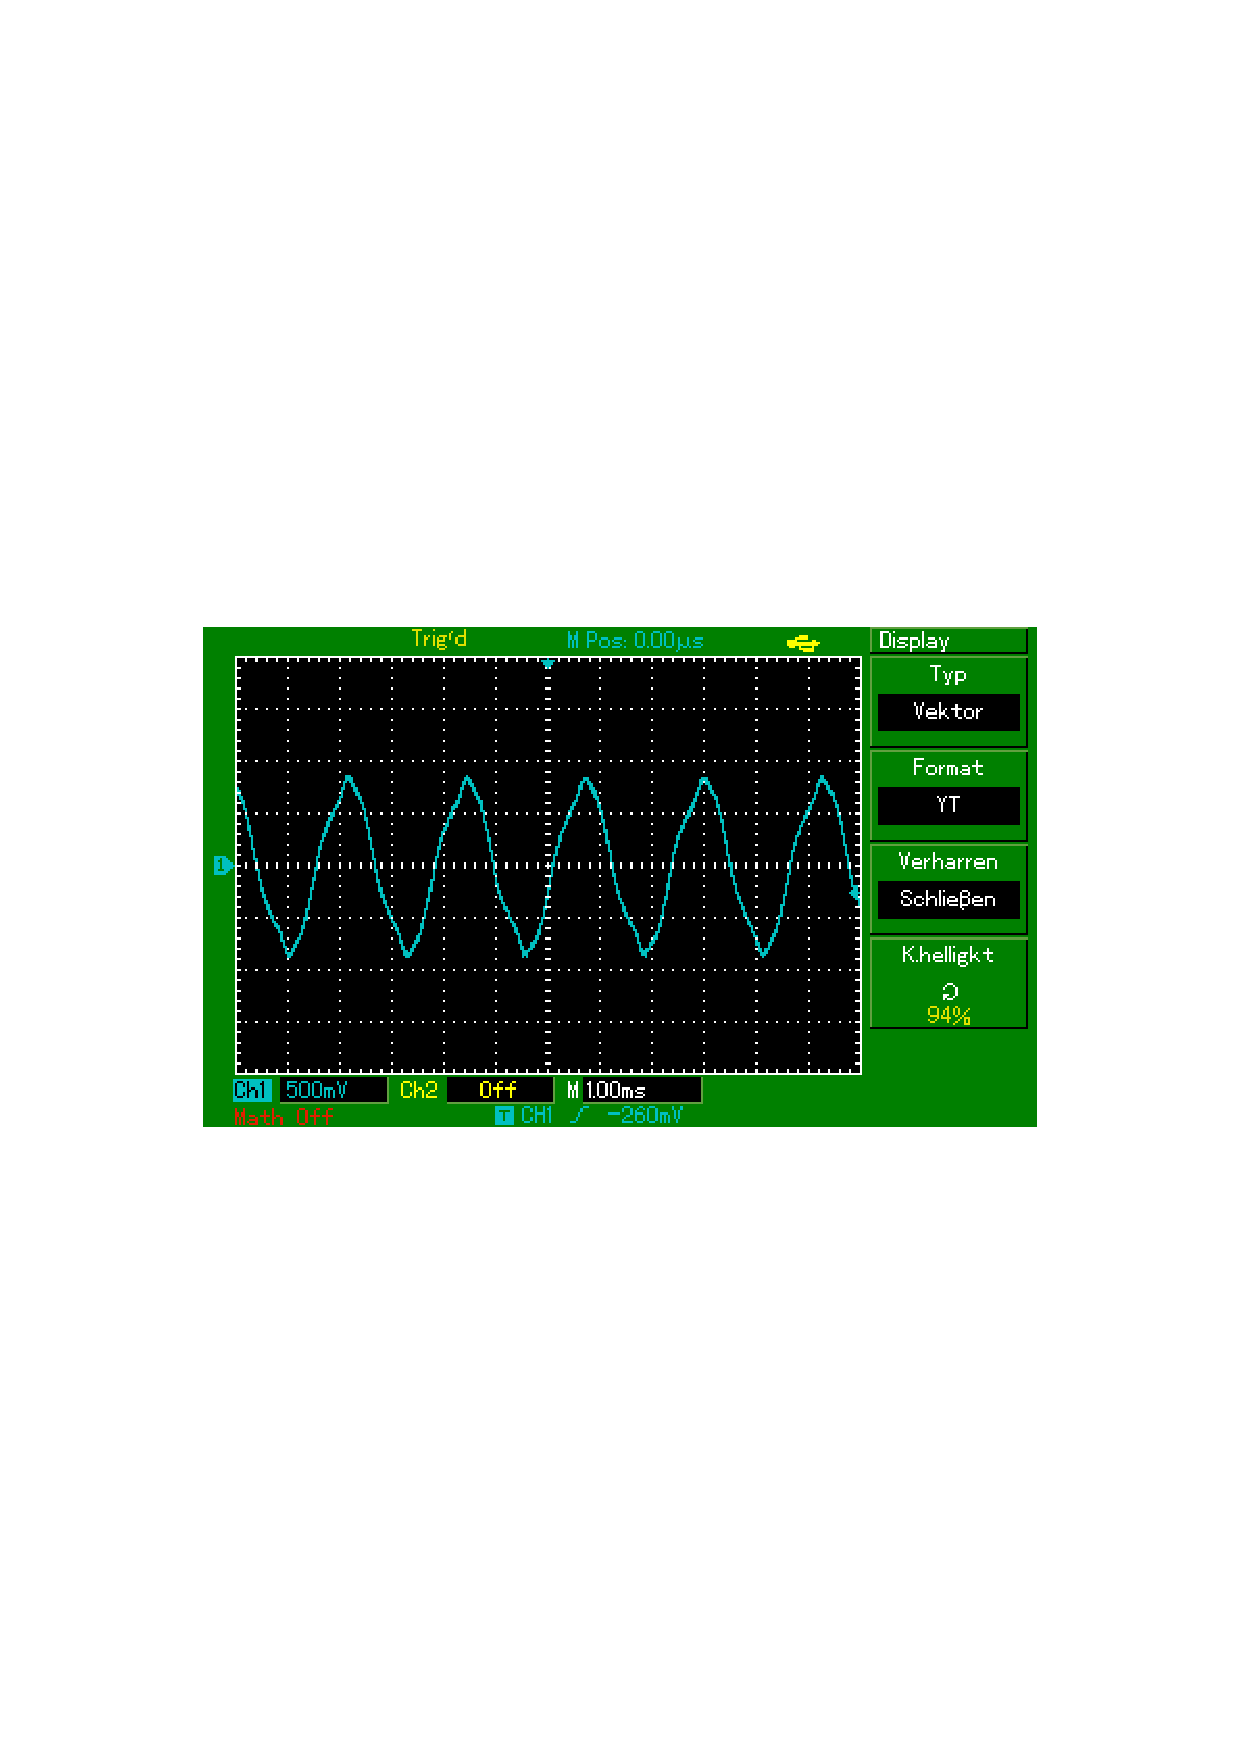
\includegraphics[scale=1.0]{content/MAP003.BMP}
%    \caption{Messwerte und lineare Regression für die Messwerte der Dreiecksspannung}
%    \label{fig:Ex3}
%\end{figure}







